\subsection{Principal Component Analysis}
\label{sub:PCA}
\subsubsection{Overview}
\label{ssub:PCAOverview}
Principal Component Analysis (PCA) is a statistical technique that can be used to identify variance in high dimensional data e.g. images.
PCA is a linear model that works by identifying the direction where most variance, i.e. change in data,
occurs and then orthogonally decomposes the variance in the other directions into vectors (See Figure~\ref{fig:pcaoverviewexample}).\\

\begin{minipage}{\linewidth}
\centering
\makebox[\linewidth] {
  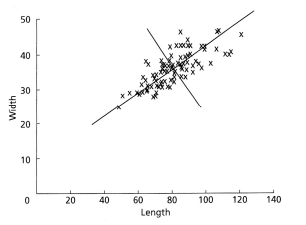
\includegraphics[width=0.5\textwidth]{PCAOverviewExample.png}
}
\captionof{figure}{Principal Component Analysis of Data in Two Dimensions\cite{holland2008pca}}\label{fig:pcaoverviewexample}
\end{minipage}\\\\

In this way, PCA allows the possibility of omitting feature vectors that have low impact on variance,
thus reducing the dimensionality of data while not loosing much of the information.

Because of the way PCA decomposes variance in orthogonal directions, it can be used as a very visual model. 
This is because the ``shape'' of the data is preserved when plotting the data using its different principal components, 
as it only requires an affine transformation from the eigenspace, the space which two principal components eigenvectors i.e. feature vectors,
to normal euclidean space.
Furthermore, this property allows the identification of linear separable patterns which can be combined with other learning techniques to
perform classification.

Another use of PCA is that it can generate images based on a means-image from the learning data and a subset of principal components.
This allows one to generate images with various weights on a principal component and identify what it actually does.

One clear disadvantage of PCA, is that it can be computationally expensive to perform on large or high-dimensional datasets.
First of all it requires the computation of a covariance matrix (see Section~\ref{ssub:HowItWorks}), which produces an array of size $n^2$, where
$n$ is the number of dimensions of data.
Then it requires calculation of eigenvectors which use the QR algorithm, which adds an additional running time of $\mathit{O}(n^3)$ \cite{abenz2012qralgorithm}.
In the end, we also work on image data which is flattened and because images usually grow proportionally in width and height this makes the data grow quadratically, i.e. $\mathit{O}(n^2)$
and the complexity is increased considerably.

\begin{minipage}{\linewidth}
\centering
\makebox[\linewidth] {
  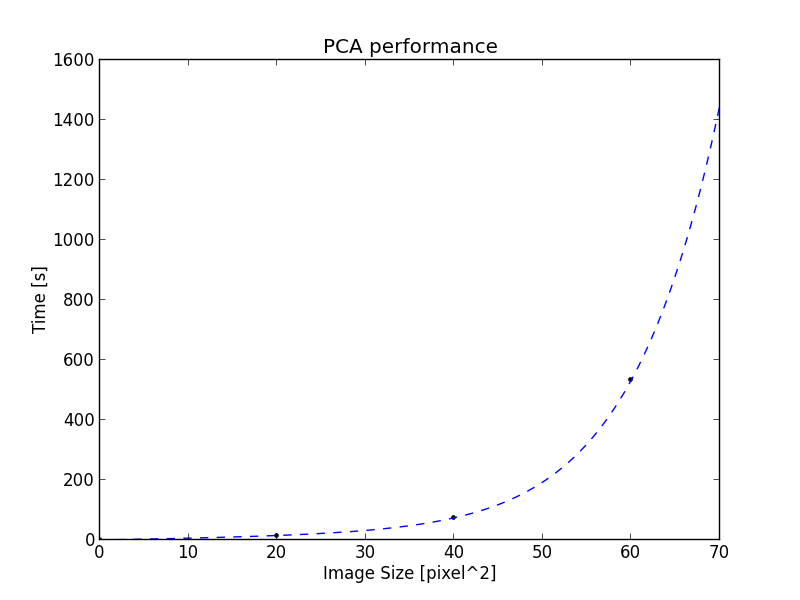
\includegraphics[width=0.5\textwidth]{pcaperformance.png}
}
\captionof{figure}{Experienced Running Time of Principal Component Analysis}\label{fig:pcarunningtime}
\end{minipage}\\\\

All these algorithms work by composition of the previous step, and thus this raises the asymptotic running time to an astounding $\mathit{O}(n^9)$.
This is an effect which we had experienced in practice where we gradually increased image size from $20 \times 20$ to $60 \times 60$ and found that on large

samples it takes almost 10 minutes to complete (See Figure~\ref{fig:pcarunningtime})\footnote{The performance test is done using an Intel Core i5-3210M dual-core processor. Because of CPU speed turbo scaling, the running times might not perform on equal conditions, and more computational intensive tasks might run faster than usual}.\\


In the following section we will explain how PCA is applied in detail. The examples are inspired by the PCA tutorial by Smith \cite{smith2002tutorial}.

\subsubsection{How It Works}
\label{ssub:HowItWorks}
\paragraph{Input data formatting.}
First of all, the data should be prepared for PCA.
In the case of images, the image should be flattened to a single vector.
This means an image of size $M$ by $N$ with $Z$ dimensions (colour values) should turn into a vector of length $M\times N\times Z$.
Turning the images into grey scale is often a good idea as it reduces the complexity by a third, and the added colour information may not be relevant.
A mean vector of all the input vectors should then be calculated and subtracted from the input vectors, producing a new input set with a mean of 0.
All of the adjusted input vectors should then be placed in a matrix where every row is an adjusted image vector.

\paragraph{Calculate the covariance matrix.}
The covariance between two dimensions can be defined as follows, assuming the mean has already been subtracted from $X$ and $Y$.
$$cov(X, Y) = \frac{\sum_{i=1}^{n} X_iY_i}{n-1}$$
The covariance should be calculated for all dimensions.
For example, for a 3 dimensional data set with dimensions $(x,y,z)$ the covariance can be calculated for $(x,y)$, $(x,z)$ and $(y,z)$.
The covariance matrix for a data set with n dimensions is defined as follows.
$$C^{n\times n} = (c_{i,j}, c_{i,j} = cov(Dim_i, Dim_j))$$
The covariance matrix for the previous imaginary data set with dimensions $(x,y,z)$ is the following.
$$
C= \begin{pmatrix}
cov(x,x) & cov(x,y) & cov(x,z) \\
cov(y,x) & cov(y,y) & cov(y,z) \\
cov(z,x) & cov(z,y) & cov(z,z) \\
\end{pmatrix}
$$
The matrix is a square $n\times n$ matrix, and is symmetrical around the main diagonal, as $cov(a,b) = cov(b,a)$.
It is also worth noting that down the main diagonal the value is the covariance between a dimension and itself.

\paragraph{Calculate eigenvectors and eigenvalues of the covariance matrix.}
Eigenvectors are vectors that when multiplied with another matrix work like a constant. For example:
$$
\begin{pmatrix}
2 & 3 \\
2 & 1
\end{pmatrix}
\times
\begin{pmatrix}
3\\
2
\end{pmatrix}
=
\begin{pmatrix}
12 \\
8
\end{pmatrix}
=
4 \times
\begin{pmatrix}
3 \\
2
\end{pmatrix}
$$
Some properties of eigenvectors: eigenvectors of a matrix can only be found for square matrices, and not every square matrix has eigenvectors. 
Given an $n\times n$ matrix that does have eigenvectors, there are $n$ of them.
The eigenvectors should be unit vectors, that being their length is exactly one.
There is no easy way to calculate eigenvectors, but most programming languages have libraries with support for calculating them.
%Skriv eventuelt mere om eigenvektorer og værdier..?

Eigenvalues are closely related to eigenvector and there was one in the previous example, namely 4.
Eigenvalues comes in pairs with eigenvectors.

\paragraph{Choosing components.}
The eigenvector with the highest eigenvalue is the principle component of the data set.
Sorting the eigenvectors by eigenvalue allows us to see what components are most important, and allows us to ignore insignificant components with low eigenvalues if necessary.
After eliminating insignificant principal components, we can then form the feature vector which is a matrix of the eigenvectors we want to keep.


\paragraph{Deriving the new data set.}
The final step of Principal Component Analysis is to apply our feature vector, $\Phi$, to the adjusted input data, $s_{input}$, where the means, $\mu_{input}$, has been subtracted.
The input data is transposed to get the data items in the columns and the dimensions in the rows.
$$s_{final} = \Phi\cdot (s_{input}-\mu_{input})^\top+\mu_{input} $$ %\top for transpose
If the means are readded, this gives us the original data expressed in terms of the patterns identified.
%Mangler at skrive om PCA i forhold til vores project?

%\paragraph{Recovering old data} virker ikke relevant
